\documentclass[mathserif]{beamer}
\usepackage[latin1]{inputenc}
\usepackage{graphicx}
\usetheme{Goettingen}
\usecolortheme{whale}

\title{Stock Price Prediction}
\author{Xiaoying Zhang \\ Lanqing Li}\institute{University of Washington}

\begin{document}

\begin{frame}
\titlepage

\end{frame}

\begin{frame}
\frametitle{Table of Contents}
\tableofcontents
\end{frame}

\section{Introduction}
\begin{frame}
\frametitle{Introduction}
The main purpose of doing this project is to predict stock price by using Java. The functions of the code we composed is that using everyday's stock price and its return as our input then we can predict the stock price and the return for the following day. We assume that the stock price and the return are standard normal distributed random variables.
\end{frame}

\section{Inputs}
\subsection{S\&P 500}
\begin{frame}
\frametitle{S\&P 500}
The S\&P 500, or the Standard \& Poor's 500, is a stock market index based on the market capitalizations of 500 large companies having common stock listed on the NYSE or NASDAQ. The S\&P 500 index components and their weightings are determined by S\&P Dow Jones Indices. It differs from other U.S. stock market indices, such as the Dow Jones Industrial Average or the Nasdaq Composite index, because of its diverse constituency and weighting methodology. It is one of the most commonly followed equity indices, and many consider it one of the best representations of the U.S. stock market, and a bellwether for the U.S. economy.
\end{frame}

\subsection{Log Return}
\begin{frame}
\frametitle{Why Use the Log of Returns, Rather Than Price or Raw Returns?}
Begin by defining a return: $r_i$ at time $i$, where $p_i$ is the price at time $i$ and $j$ $\equiv$ $(i - 1)$:

\[r_i = \frac{p_i - p_j}{p_i}\]

First, {\em log-normality}: if we assume that prices are distributed log normally (which, in practice, may or may not be true for any given price series), then $log(1 + r_i)$ is conveniently normally distributed, because:
\[1 + r_i = \frac{p_i}{p_j} = e^{log(\frac{p_i}{p_j})}\]
This is handy given much of classic statistics presumes normality.
\end{frame}

\begin{frame}
\frametitle{Why Use the Log of Returns, Rather Than Price or Raw Returns?}
Second, {\em approximate raw-log equality}: when returns are very small (common for trades with short holding durations), the following approximation ensures they are close in value to raw returns:
\[log(1 + r) \approx r , r \ll 1 \]
\end{frame}

\begin{frame}
\frametitle{Why Use the Log of Returns, Rather Than Price or Raw Returns?}
Third, {\em time-additivity}: consider an ordered sequence of $n$ trades. A statistic frequently calculated from this sequence is the compounding return, which is the running return of this sequence of trades over time:
\[log(1 + r_i) = log(\frac{p_i}{p_j}) = log(p_i) - log(p_j) \]
Thus, compounding returns are normally distributed. 
\end{frame}

\begin{frame}
\frametitle{Why Use the Log of Returns, Rather Than Price or Raw Returns?}
Finally, this identity leads us to a pleasant algorithmic benefit; a simple formula for calculating compound returns:
\[\sum_{i}^n log(1+r_i) = log(1 + r_1) + log(1 + r_2)  + \cdots + log(1 + r_n) \] \[= log(p_n) - log(p_0)\]
Thus, the compound return over n periods is merely the difference in log between initial and final periods. 
\end{frame}

\begin{frame}
\frametitle{Why Use the Log of Returns, Rather Than Price or Raw Returns?}
In terms of {\bfseries algorithmic complexity}, this simplification reduces $O(n)$ multiplications to $O(1)$ additions. This is a huge win for moderate to large $n$. Further, this sum is useful for cases in which returns diverge from normal, as the {\bfseries central limit theorem} reminds us that the sample average of this sum will converge to normality (presuming finite first and second moments).
\end{frame}

\section{Outputs}
\begin{frame}
\frametitle{Outputs}
    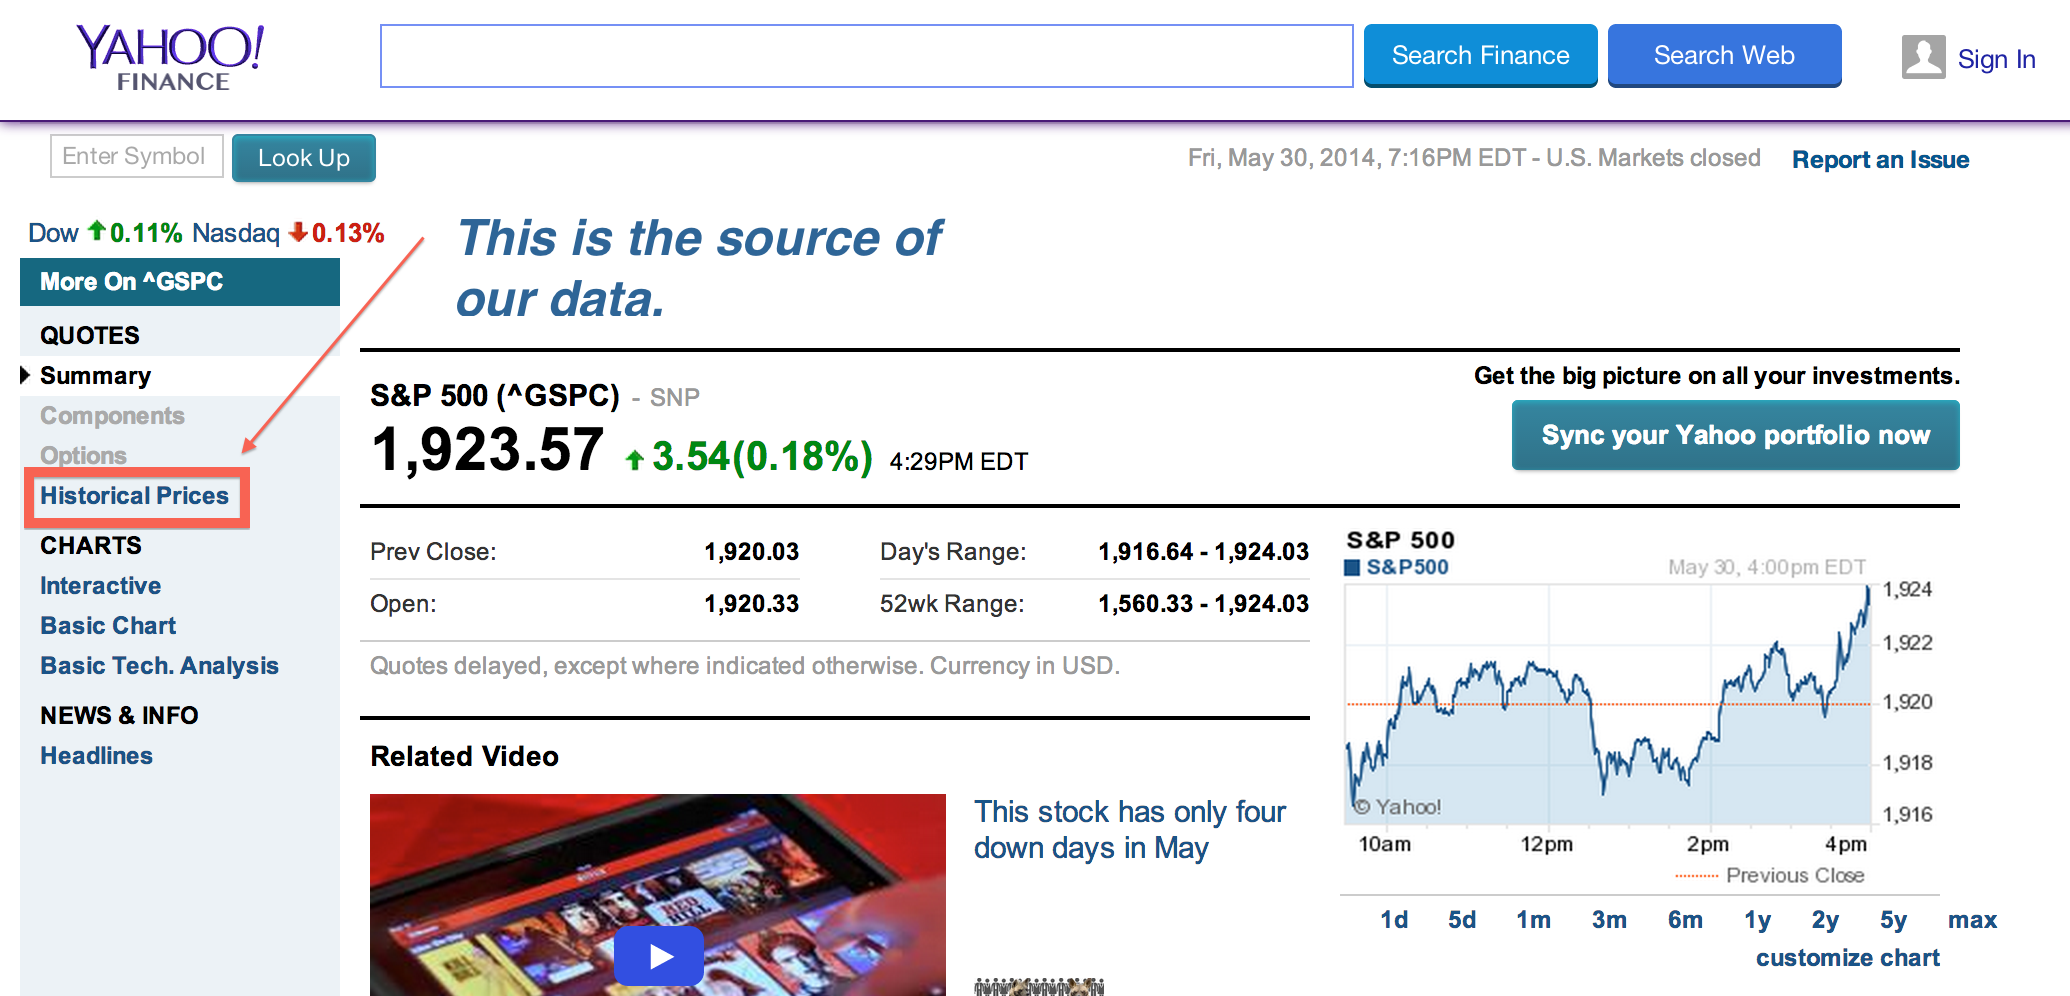
\includegraphics[height=5cm]{5.png}
\end{frame}

\section{Visualized Result}
\begin{frame}
\frametitle{Visualized Result}
    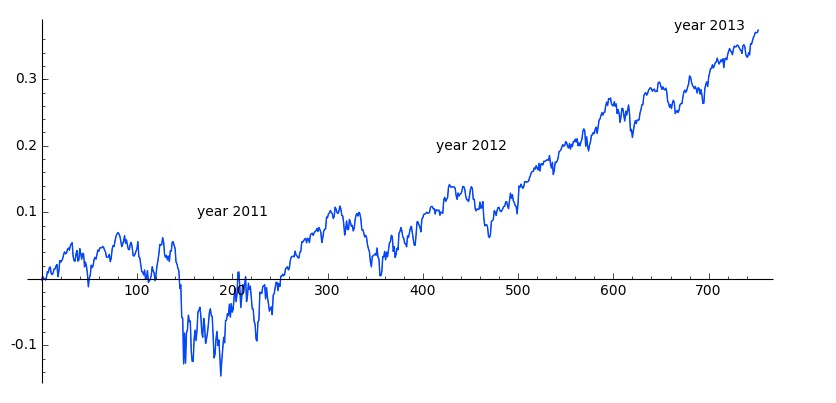
\includegraphics[height=4cm]{1.jpg}
\end{frame}

\begin{frame}
\frametitle{Visualized Result}
    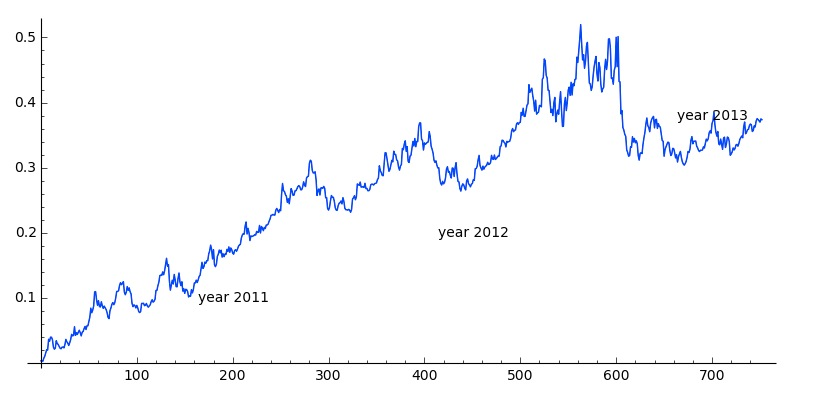
\includegraphics[height=4cm]{2.jpg}
\end{frame}

\begin{frame}
\frametitle{Visualized Result}
    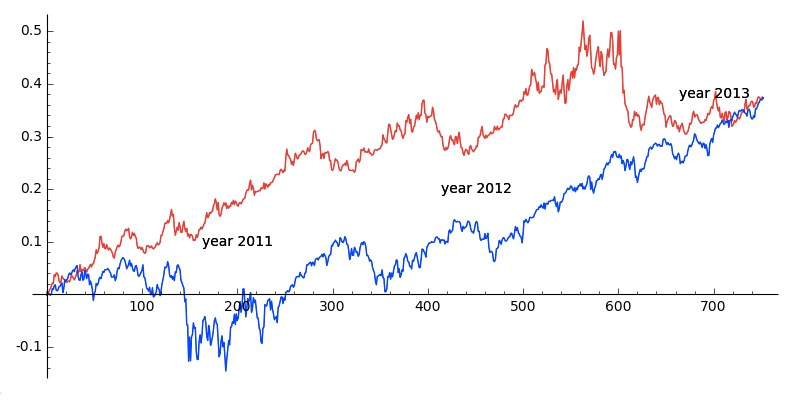
\includegraphics[height=5cm]{3.jpg}   
\end{frame}

\begin{frame}
\frametitle{Realtime Graph}
    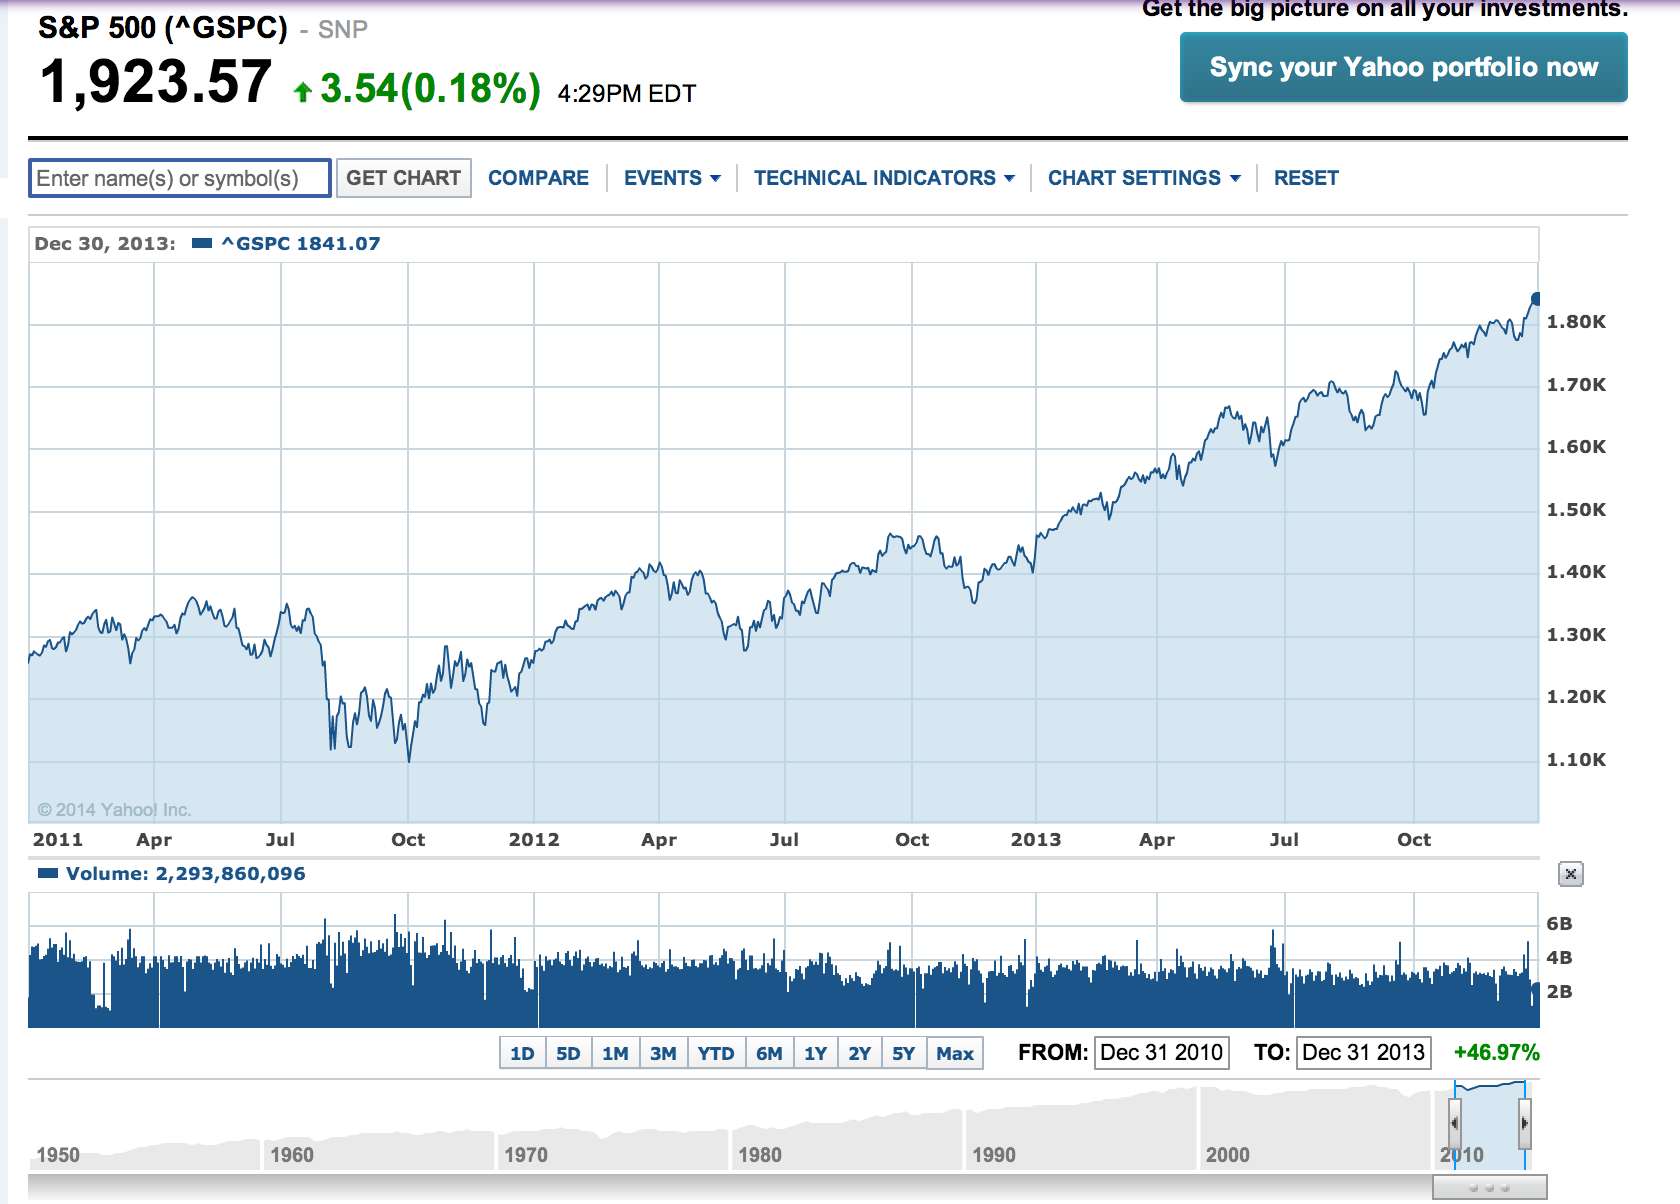
\includegraphics[height=7cm]{4.png}   
\end{frame}

\section{Flaws}
\begin{frame}
\frametitle{Flaws of the Project}
Real stock market involves tons of elements that can change the stock price, such as 911 leading to a quick drop of stock price. This shows us that accident that no one can anticipate will effect the stock price dramatically. And the random sector that we are using is standard normal distribution. We assume that the stock price will change within the range of this standard normal distribution. However, this will not be the case of real life. Also, the policy maker may make some rules that can also effect the stock price. Thus, we assume that non of above will happen and stock price will change in the range of standard normal distribution. This is only a roughly and ideal way to anticipate the stock price. 
\end{frame}

\end{document}
%sagemathcloud={"zoom_width":90}